% Section facultative mais importante à mon avis

% 2 points clé : la méthodologie et pourquoi ce choix de technique
\section{Bayesian model}
\label{section:bayesmodel}
To solve this problem, the approach taken is a non-parametric Bayesian model based on the \textit{Hidden Markov Model} and a prior generated by a \textit{Hierarchical Dirichlet Process} (HDP-HMM). We want to segment a waveform into a set of time intervals with no \textit{a priori} on the number of intervals. The sequence is modelled using the Hidden Markov Model with the states to categorise the interval. In other words, we want the piece to be divided into intervals and each interval will be labelled to a state that we will later on analyse. For example a music piece can be divided into parts that are : intro, chorus, pre-chorus, outro. Those parts can be easily identified by the human ear and brain (music-theoretic analysis). We will compare our analysis to the results of the model. 

\begin{figure}[ht]
	\label{fig:waveform}
	\centering
  	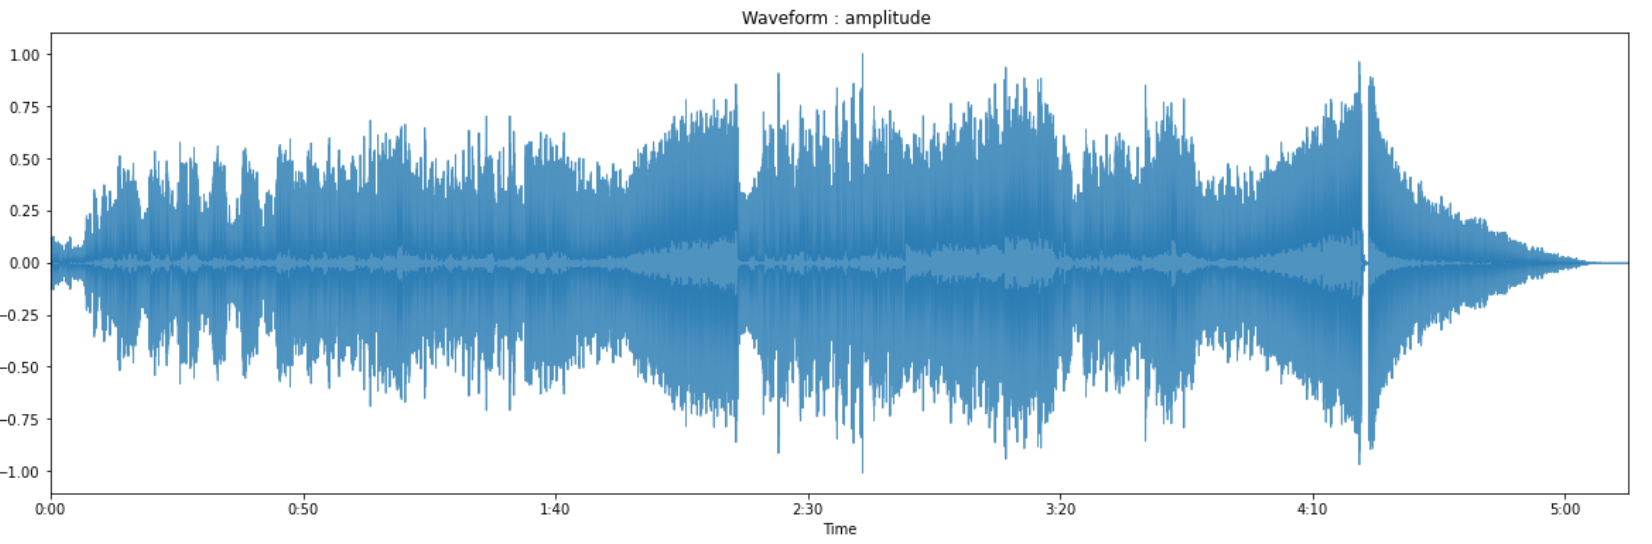
\includegraphics[scale=0.5]{Graphics/Audio/waveform2} 
   	\caption{Audio waveform of the piece considered}
\end{figure}

\subsection{Hidden Markov Model}
The Hidden Markov Model used is described as follows : A discrete sequence of observed data $x=\{x_t\}^T_{t=1}$ with $x_t \in \{1,\dots, M \}$ and a corresponding hidden state sequence $s=\{s_t\}^T_{t=1}$ with $s_t \in \{ 1, \dots, I \}$. The states will be analysed as in Section \ref{section:bayesmodel} (intro, chorus, etc.). Each observation is associated to a state. The discrete HMM model is represented by its parameters $\theta=\{A,B,\pi\}$ such that : 
\begin{itemize}
	\item $A$ is a set of state transition probabilities, the probability to transition from one state to another.For two states $\rho$ and $\xi$, the transition probability from $\rho$ to $\xi$ is $a_{\rho\xi}=\mathbb P(s_{t+1}=\xi | s_t=\rho)$
	\item $B$ is a set of emission probabilities, the probability that an observation associated to a state $\rho$ is equal to $m$ : $b_{\rho m}=\mathbb P(x_t= m | s_t=\rho)$
	\item  $\pi$ is the set of initial state distribution, the probability that the first observation in time $t=1$ is equal to the state $\rho$ : $\pi_{\rho}=\mathbb P(s_1=\rho)$
\end{itemize}
Because we will use a Hierchical Dirichlet Process to model the parameters $\theta$, we will divide the sequence into $J$ subsequences. This means that we will model J Hidden Markov Models. By taking the notation at the beginning of this section, we will have $j\in \{1, \dots, J\}$ and $x=\{x_j\}_{j=1}^J$ with $x_j=\{ x_{jt}\}_{t=1}^T$. Note that the total length of the discrete sequence is $J\times T$ and every subsequence $x_j$ has a length T. We allow the parameters to be different in each subsequence such that : \begin{align*}
 		x_j \sim HMM(\theta_j)
 \end{align*}
The joint distribution given $\theta$ is : 
\begin{align*}
	p(x|\theta)=\prod^J_{j=1}\left\{ \sum_{s_j}\pi_{{j,1}}\prod^{T-1}_{t=1}a_{s_{j,t+1}} \prod^T_{t=1} b_{s_{j,t}x_{j,t}} \right\}
\end{align*}

\subsection{Hierchical Dirichlet Process}
A Hierchical Dirichlet Process is defined as a collection of Dirichlet Processes. Our collection of DP processes is the J parameters $\theta_j$ linked to the HMM. This kind of setting allows for analysing how inter-related are the subsequences one to the others. The first process of the collection is denoted as : 
\begin{align*}
	G_0\sim DP(\gamma, H)
\end{align*}
with $\gamma$ a concentration parameter for the Dirichlet distribution which is symmetrical and H a base probability measure on $\Theta$. The formal definition of a Dirichlet process is $\forall (B_k)_{k=1,\dots, K}$ finite partition of $\Theta$ : \begin{align*}
	(G_0(B_k))_{k=1,\dots, K}|\gamma, H \sim Dir( (\gamma H(B_k))_{k=1,\dots, K})
\end{align*}
We approach the Dirichlet Process with a stick-breaking process and we can write $G_0$ as follows :
\begin{align*}
	G_0=\sum^\infty_{k=1} \beta_k \delta_{\theta_k}
\end{align*}
with $\delta_{\theta_k}$ an indicator function in $\theta_k$ and $\beta_k$ the mixture weights computed such that :
\begin{align*}
\beta_k &\sim Stick(\gamma) \\
	\beta_k&= v_k\prod^{k-1}_{l=1}(1- v_l) \\
	v_k&\sim Beta(1, \gamma)
\end{align*}
with $v_k$ the independent random variables following a Beta distribution. The process to obtain the probabilities $\beta_k$ is pictured as breaking a unit-length stick because we start off with a stick of length 1 and at each step we  we break a portion of the what is remaining stick according to $v_k$ and assign to $\beta_k$ the piece broken. The smaller the $\alpha$ the more concentrated is the distribution. The first process $G_0$ is then used as the base measure for the other processes : \begin{align*}
	G_j \sim DP(\alpha, G_O)
\end{align*} 
In our case we consider : 
\begin{align*}
	\theta_i' \sim G_0
\end{align*}



\section{Data processing}
We consider an acoustic signal in a mp3 format loaded in Python using the librosa package. The sampling rate is 22.05kHz which means we have 22050 observations par second of audio signal. The acoustic signal is first loaded as a waveform or amplitude as shown in Figure \ref{fig:waveform}. It represents the pressure change recorded by a recording instrument such as a microphone. We then divide the piece into 100ms contiguous frames. Each amplitude frame is processed by computing its Mel frequency sceptral coefficients (MFCCs). These coefficients are derived from the Melspectrogram that is a log-scale of pitches judged to be equally distanced to one another. The Mel spectrogram is the representation showing the mel frequencies according to time and intensity. The MFCCs are the most popular feature used in audio processing. We compute 40 columns of coefficients for each frame. To obtain a vector sequential data, we quantize each frame of coefficient. First, we \textit{whiten} the columns so each one of them have a unit variance. Then we use the k-means algorithm with 16 codebooks and pass them to the vector quantization algorithm. The result is a 1D discrete sequential data representing the coefficients. 



\section{Computational method}
% 2 points clé : la description de la méthode et les difficultés rencontrées

\section{Results}
% 2 points clé : l'explication des résultats et l'interprétation

